%% $RCSfile: proj_report_outline.tex,v $
%% $Revision: 1.3 $
%% $Date: 2016/06/10 03:41:54 $
%% $Author: kevin $

\documentclass[11pt
              , a4paper
%%              , twoside
              , openright
              ]{report}


\usepackage{float} % lets you have non-floating floats

\usepackage{url} % for typesetting urls
\usepackage{amsmath}
\usepackage{amsthm}
\usepackage{amssymb}
\usepackage{float}
\usepackage{graphicx}
\usepackage{subfig}
\usepackage[utf8]{inputenc}
\usepackage[english]{babel}
\usepackage[linesnumbered,ruled]{algorithm2e}
\usepackage[toc,page]{appendix}
\usepackage{listings}
\usepackage{soul}

\usepackage[usenames, dvipsnames]{color}


\theoremstyle{definition}
\newtheorem{definition}{Definition}[section]
\newtheorem{theorem}{Theorem}[section]
\newtheorem{conjecture}{Conjecture}[section]

\definecolor{grey}{rgb}{0.95,0.95,0.95}

\lstset{ %
	backgroundcolor=\color{grey},
	frame=single,
	numbers=left
}
\newcommand{\code}[1]{\texttt{#1}}

\newcommand{\comment}[1]{
	{\color{red} \fbox{\parbox{\textwidth}{{\color{ForestGreen} #1}}}}
}

%
%  We don't want figures to float so we define
%
\newfloat{fig}{thp}{lof}[chapter]
\floatname{fig}{Figure}

%% These are standard LaTeX definitions for the document
%%                            
\title{Logical Neural Networks: Opening the black box}
\author{Daniel Thomas Braithwaite}

%% This file can be used for creating a wide range of reports
%%  across various Schools
%%
%% Set up some things, mostly for the front page, for your specific document
%
% Current options are:
% [ecs|msor|sms]          Which school you are in.
%                         (msor option retained for reproducing old data)
% [bschonscomp|mcompsci]  Which degree you are doing
%                          You can also specify any other degree by name
%                          (see below)
% [font|image]            Use a font or an image for the VUW logo
%                          The font option will only work on ECS systems
%
\usepackage[image,ecs,bschonscomp]{vuwproject}

% You should specifiy your supervisor here with
     \supervisor{Marcus Frean}
% use \supervisors if there is more than one supervisor

% Unless you've used the bschonscomp or mcompsci
%  options above use
%   \otherdegree{OTHER DEGREE OR DIPLOMA NAME}
% here to specify degree

% Comment this out if you want the date printed.
\date{}

\begin{document}

% Make the page numbering roman, until after the contents, etc.
\frontmatter

%%%%%%%%%%%%%%%%%%%%%%%%%%%%%%%%%%%%%%%%%%%%%%%%%%%%%%%

%%%%%%%%%%%%%%%%%%%%%%%%%%%%%%%%%%%%%%%%%%%%%%%%%%%%%%%

\begin{abstract}
Artificial Neural Networks are growing in popularity and can generalise well to unseen examples. However it can be difficult to interpret the learned models. A problem which is driving the development of systems that are not only accurate but have a decision-making process that can be defended. This report develops a novel neural network architecture which builds in an interpretable structure. Experiments on the MNIST dataset showed these models had statistically equivalent performance to Multi-Layer Perceptron Networks and provided evidence that they have a more interpretable learned model. The networks developed here were also shown to perform well when compared with recently developed methods aimed at solving the same problem.

\end{abstract}

%%%%%%%%%%%%%%%%%%%%%%%%%%%%%%%%%%%%%%%%%%%%%%%%%%%%%%%

\maketitle

\chapter*{Acknowledgements}
\thispagestyle{empty}

I would like to acknowledge my supervisor Marcus Frean for the continued support helping me achieve a research project I can be proud of


\tableofcontents

% we want a list of the figures we defined
%\listof{fig}{Figures}

%%%%%%%%%%%%%%%%%%%%%%%%%%%%%%%%%%%%%%%%%%%%%%%%%%%%%%%

\mainmatter

%%%%%%%%%%%%%%%%%%%%%%%%%%%%%%%%%%%%%%%%%%%%%%%%%%%%%%%

% individual chapters included here
\chapter{Introduction}\label{C:intro}
Artificial Neural Networks (ANN's) are commonly used to model supervised learning problems. NN's often achieve higher accuracy than other methods because they are able to approximate any continuous function. A well trained NN can generalize well but it is very difficult to interpret how the network is operating, this is called the black-box problem. \\

The growing number of situations in which ANN systems are used has lead to an increasing interest in systems which are not only accurate but also provide explanations of there answers \cite{doshi2017towards}. This increasing interest is driven by the verity of applications of ANNs where incorrect or biases answers can have significant effects on users.\\

Safety and ethics are two concrete examples of such situations where explanations of reasoning would provide a method to ensure an ANN can be implement with mitigated risk \cite{doshi2017towards}. In the context of Safety an ML system often can not be tested against all possible situations as it is computationally infeasible, the reasoning the ML system uses could be examined for flaws that could be result in a failure \textbf{Example Here}. On the other hand it is important to consider the implications of an ANN being biased towards a protected class of people, \textbf{Example Here}\\

Another pressure causing the development of this field is changing laws, in 2018 a European Union (EU) regulation will come into effect requiring algorithms which  profile users based on their personal information have the right to "Meaningful information about the logic involved" \cite{goodman2016european} \textbf{Cite LAW HERE}.\\

Growing applications and changing laws are applying pressure to the field of Machine Learning to develop more intepretable systems. This report develops a new network archetchure which yields an intepretable trained model. This model is derived by first considering the descrete space of boolean algeabra and defining a class of networks to learn Conjunctive and Disjunctive Normal Forms of boolean formula,

ANNs are black-boxes \textbf{REFERNECE}








Consider some function $f$, then the operation of restricting a neuron to $f$ is given by only allowing a function given by $f$ operating on the set of weighted inputs (each input multiplied by a corresponding weight) to be learnt. By restricting the function set that each neuron can learn is it possible to create a more interpretable network? This report develops a class of networks where the function space of each neuron is restricted to be a predefined operation which can be interpreted as Boolean expression i.e. an AND or OR of its inputs.\\

Boolean functions are by nature discrete, as such do not have a continuous differential, making them unsuitable for training with an algorithm such as Backpropagation. This report makes use of Noisy-OR and Noisy-AND neurons \cite{LearningLogicalActivations}, which are generalized continuous parametrisations of OR and AND gates.\\

ANN's consisting of Noisy neurons are called Logical Neural Networks (LNN's). LNN's have been used to classify the MINST dataset with promising results, while not being able to achieve a state of the art accuracy they have been shown to yield simpler (sparser) and more interpretable weight vectors \cite{LearningLogicalActivations}. It was also shown that using Noisy neurons in combination with standard sigmoid units results in poor performing networks without the benefit of being more interpretable \cite{LearningLogicalActivations}, for this reason networks of this kind are not considered.\\

This report takes a different approach to using these interpretable Noisy neurons, instead they are placed in specific configurations which allow learning Conjunctive or Disjunctive Normal Form expressions, these are called Logical Normal Form Networks (LNFN's) and are a subset of LNN's.\\

This report demonstrates by experimentation that when provided a complete truth table for a boolean expression, the performance of LNFN's has no statistically significant differences to that of a Multi-Layer Perceptron (MLPN) Network. The LNFN's are also able to generalize, obtaining statistically equivalent performance to a MLPN when given incomplete truth tables.\\

By inspecting the weights of each Noisy neuron it is possible to determine a relationship between the inputs and output. Rule extraction algorithms exist as a method to extract knowledge from NN's \cite{andrews1995survey}, if LNFNs are more interpretable then are rules able to be extracted from them? When first considering problems with Boolean inputs and outputs, if a low enough error is achieved when training an LNFN over a complete truth table, it is possible to extract boolean rules from each neuron, consequently it is possible to obtain a boolean expression which represents the ANN and original truth table. Training over entire a complete data set is an unlikely scenario, this report investigates what effect training with incomplete truth tables has on any extracted formula. Only being able to apply LNFNs to Boolean problems does not make them very useful, this report investigates ways these networks can be applied to problems with inputs in a continuous domain.\\

The restriction placed on the function space of each neuron, while improving the interpretability, intuitively will also hinder their ability to be universal approximators. Along with the investigation of LNFNs and their potential, the limitations are also explored.


\chapter{Background}\label{C:backgroundsurvey}
\section{Related Work}
\subsection{Rule Extraction}

A survey in 1995 focuses on rule extraction algorithms \cite{andrews1995survey}, identifying the reasons for needing these algorithms along with introducing ways to categorise and compare them.\\

There are three categories that rule extraction algorithms fall into \cite{andrews1995survey}. An algorithm in the \textbf{decompositional} category focuses on extracting rules from each hidden/output unit. If an algorithm is in the \textbf{pedagogical} category then rule extraction is thought of as a learning process, the ANN is treated as a black box and the algorithm learns a relationship between the input and output vectors. The third category, \textbf{electic}, is a combination of decompositional and pedagogical. Electic accounts for algorithms which inspect the hidden/output neurons individually but extracts rules which represent the ANN globally \cite{tickle1998truth}.\\

To further divide the categories two more distinctions are introduced. One measures the portability of rule extraction techniques, i.e. how easily can they be applied to different types of ANN's. The second is criteria to assess the quality of the extracted rules, these are accuracy, fidelity, consistency, comprehensibility \cite{andrews1995survey}.

\begin{enumerate}
\item A rule set is \textbf{Accurate} if it can generalize, i.e. classify previously unseen examples.
\item The behaviour of a rule set with a high \textbf{fedelity} is close to that of the ANN it was extracted from.
\item A rule set is \textbf{consistent} if when trained under different conditions it generates rules which assign the same classifications to unseen examples.
\item The measure of \textbf{comprehensibility} is defined by the number of rules in the set and the number of literals per rule.
\end{enumerate}

One rule extraction algorithm presented in 2000 by Tsukimoto is able to extract boolean rules from ANNs in which neurons have monotonically increasing activations, such as the sigmoid function \cite{tsukimoto2000extracting}. The algorithm can be applied to problems with boolean or continuous inputs however only the boolean case will be considered here.\\

Each neuron is written as a boolean operation on its inputs, this is done in the following manner. Consider a neuron $m$ in an MLPN with $n$ inputs, construct a truth table, T, with $n$ inputs. Let $f_i (i \in [0, 2^n])$ represent the activation of $m$ when given row $i$ as input and define $r_i = \land_{j=1}^{n} l_j$, the conjunction of all literals in the row $i$ in T, e.g. if $n=2$ then for row $(1,0)$ $r_i = x_1 \land \lnot x_2$. The approximation of $m$ is given by 

\begin{align}
	\lor_{i=1}^{2^n}\ g_i \land r_i
\end{align}

where $g_i$ is given by

\[
g_i =
\begin{cases}
1 & \text{if $f_i \geq \frac{1}{2}$} \\
0 & \text{if $f_i < \frac{1}{2}$} \\
\end{cases}
\]

By starting with the first hidden layer and progressing through the network an expression for the network can be extracted. Figure \ref{alg:rule-extraction-tsukimoto} shows an algorithm for extracting rules from an MLPN.

\begin{figure}[H]
\begin{lstlisting}[mathescape=true]
function extractRulesMLPN(network)
  prev_expressions = network.inputs
  for layer in network
    expressions = {}
    patters = all input patters for layer
    for each neuron (n) in layer
      exp = And(Or({literals(p), $p \in $patterns n(p) > $\frac{1}{2}$}))
      expressions.add(substitute prev_expressions into exp)
	  
    prev_expressions = expressions
\end{lstlisting}
	\caption{Rule Extraction Algorithm presented in \cite{tsukimoto2000extracting}}
	\label{alg:rule-extraction-tsukimoto}
\end{figure}

The algorithm presented in figure \ref{alg:rule-extraction-tsukimoto} is certainly exponential time in terms of $n$, a polynomial time algorithm is also presented but deriving such an algorithm is beyond the scope of this report.\\

These rule extraction algorithms are all post-hoc operations. They do not place many restrictions on the structure of ANN they are applied to, resulting with complicated algorithms. The solution developed in this report builds intepretability into the ANN structure with the goal of simpler and more intuitive algorithms to interpret knowledge.

\subsection{LIME}
\comment{Talk about LIME algorithm here}

\section{Noisy Neurons} \label{sec:background-noisy-neurons}
MLPNs are universal function approximators and as such can achieve a high accuracy across a broad range of problems. There are many equivalent weight representations of an MLPN which give the same solutions, this makes interpreting the network difficult \cite{LearningLogicalActivations}. By restricting the possible relationships between a neurons inputs and outputs the problem interpretation becomes easier. The two functions OR and AND are easy to understand, a good reason to pick them over other functions.\\
 
In 2016 the concept of Noisy-OR and Noisy-AND neurons where developed \cite{LearningLogicalActivations}. Noisy neurons are derived from the Noisy-OR relation\cite{LearningLogicalActivations}, developed by Judea Pearl \cite{russell1995modern}, a concept in Bayesian Networks. A Bayesian Network represents the conditional dependencies between random variables in the form of a directed acyclic graph.

\begin{figure}[H]
	\centering
	\begin{minipage}[b]{0.4\textwidth}
		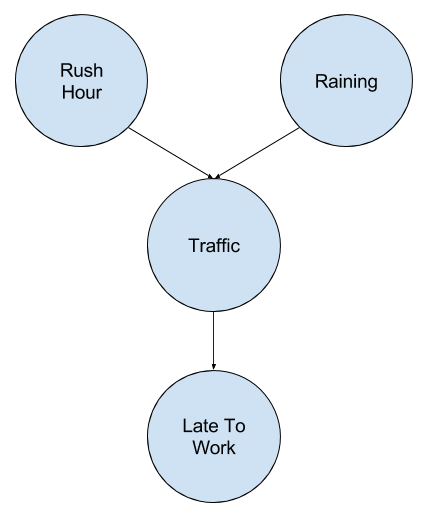
\includegraphics[width=\textwidth]{bayesian-network-example.png}
		\caption{}
		\label{fig:bayesian-network-example}
	\end{minipage}
	\hfill
\end{figure}

Figure \ref{fig:bayesian-network-example} is a Bayesian network, it demonstrates the dependency between random variables "Rush Hour", "Raining", "Traffic", "Late To Work". The connections show dependencies i.e. Traffic influences whether you are late to work, and it being rush hour or raining influences whether there is traffic.\\

Consider a Bayesian Network having the following configuration, take some node $D$ with $S_1,..., S_n$ as parents i.e. $S_i$ influences the node $D$, each $S_i$ is independent from all others. The relationship between D and its parents is if $S_1\ OR\ ...\ OR\ S_n$ is true then $D$ is true. Let $\epsilon_i$ be the uncertainty that $S_i$ influence $D$ then $P(D = 1| S_1 = 1, , S_n = 1)$ can be defined.

\begin{align}
P(D = 1 | S_1 = 1, ..., S_n = 1) = 1 - \prod^n_{i=1} \epsilon_i
\label{equ:noisy-or-relation}
\end{align}

Equation \ref{equ:noisy-or-relation} shows the noisy or relation \cite{LearningLogicalActivations}. In the context of a neuron, the inputs $x_1, ..., x_n$ represent the probability that inputs $1, ..., n$ are true. Consider the output of a neuron as conditionally dependent on the inputs, in terms of a Bayesian Network each $x_i$ is a parent of the neuron. Each $\epsilon_i$ is the uncertainty as to whether $x_i$ influences the output of the neuron. How can weights and inputs be combined to create a final activation value for the neuron. First consider a function $f(\epsilon, x)$ which computes the irrelevance of input x. Some conditions that can be placed on $f$ are given in \cite{LearningLogicalActivations}. (1) $\epsilon = 1$ means that $f(\epsilon, x) = 1$, (2) $x = 1$ means that $f(\epsilon, x) = 1$, (3) Monotonically increasing in $\epsilon$ and decreasing in x. Let $f(x, \epsilon) = \epsilon^x$. The definitions for Noisy-OR and Noisy-AND gates can now be given.

\begin{definition}
	A \textbf{Noisy-OR} Neuron has weights $\epsilon_1, ..., \epsilon_n \in (0,1]$ which represent the irrelevance of corresponding inputs $x_1, ..., x_n \in [0,1]$. The activation of a Noisy-OR Neurons is.
	
	\begin{align}
	a = 1 - \prod^p_{i=1} (\epsilon_i^{x_i}) \cdot \epsilon_b
	\label{equ:noisy-or-activation-1}
	\end{align}
\end{definition}

\begin{definition}
	A \textbf{Noisy-AND} Neuron has weights $\epsilon_1, ..., \epsilon_n \in (0, 1]$ which represent the irrelevance of corresponding inputs $x_1, ..., x_n \in [0,1]$. The activation of a Noisy-AND Neurons is.
	
	\begin{align}
	a = \prod^p_{i=1} (\epsilon_i^{1 - x_i}) \cdot \epsilon_b
	\label{equ:noisy-and-activation-1}
	\end{align}
\end{definition}

Both these parametrisations reduce to discrete logic gates when there is no noise, i.e. $\epsilon_i = 0$ for all $i$.\\

\section{Logical Neural Networks}
ANN's containing of Noisy-OR and Noisy-AND neurons are called Logical Neural Networks (LNN's), if the network consists of only Noisy neurons then it a pure LNN. LNN's have been applied to the MINST dataset with promising results. Experiments with different combinations of logical and standard (sigmoid, soft-max) neurons have shown that pure LNN's where able to achieve an error of 8.67\%, where a standard perceptron/softmax network was able to achieve an error of 3.13\%. This reduction in performance does not come without reward, the pure LNN yields a simpler (sparser) and more interpretable network \cite{LearningLogicalActivations}. Training LNN's which are not pure have been shown to have reduced performance (compared to standard ANN's) and no interpretability benefit.\\

\section{CNF \& DNF}
A boolean formula is in Conjunctive Normal Form (CNF) if and only if it is a conjunction (and) of clauses. A clause in a CNF formula is given by a disjunction (or ) of literals. A literal is either an atom or the negation of an atom, an atom is one of the variables in the formula.\\

Consider the boolean formula $\lnot a \lor (b \land c)$, the CNF is $(\lnot a \lor b) \land (\lnot a \lor c)$. In this CNF formula the clauses are $(\lnot a \lor b)$, $(\lnot a \lor c)$, the literals used are $\lnot a$, $b$, $c$ and the atoms are $a$, $b$, $c$.\\

A boolean formula is in Disjunctive Normal Form (DNF) if and only if it is a disjunction (or) of clauses. A DNF clause is a conjunction (and) of literals. Literals and atoms are defined the same as in CNF formulas.\\

Consider the boolean formula $\lnot a \land (b \lor c)$, the DNF is $(\lnot a \land b) \lor (\lnot a \land c)$.\\

\subsection{CNF \& DNF from Truth Table} \label{subsec:construct-cnfdnf}
Given a truth table representing a boolean formula, constructing a DNF formula involves taking all rows which correspond to True and combining them with an OR operation. To construct a CNF one combines the negation of any row which corresponds to False by an OR operation and negates it.

\begin{theorem}
	The maximum number of clauses in a CNF or DNF formula is $2^n$
	\label{thm:max-clause-cnfdnf}
\end{theorem}

\begin{proof}
	Assume the goal is to find the CNF and DNF for a Boolean formula B of size $n$, for which the complete truth table is given. The truth table has exactly $2^n$ rows.\\
	
	First assume a CNF is being constructed, this is achieved by taking the OR of the negation of all rows corresponding to False, the NOT operation leaves the number of clauses unchanged. At most there can be $2^n$ rows corresponding to False, consequently there are at most $2^n$ clauses in the CNF.\\
	
	A similar argument shows that the same holds for DNF.
\end{proof}

\section{Logical Normal Form Networks}
In 1996 a class of networks, called Logical Normal Form Networks (LNFNs), where developed \cite{herrmann1996backpropagation}, focusing on learning the underlying CNF or DNF for a boolean expression which describes the problem. The approach relies on a specific network configuration along with restriction the function space of each neuron, allowing them to only perform an OR or AND on a subset of their inputs, such OR and AND neurons are called Disjunctive and Conjunctive retrospectively. If the trained network is able to achieve a low enough accuracy then rules can be extracted from the network in terms of a Boolean CNF or DNF expression \cite{herrmann1996backpropagation}.\\

The algorithm which extracts rules from LNFNs would be Electic and certainly is not Portable as the algorithm is specific to the LNFN architecture. It is not possible to further classify the rule extraction algorithm as the research developing it lacks any experimental results, much justification is also missing making the LNFNs difficult to reproduce.\\



\chapter{Logical Normal Form Networks}\label{C:workdone}
Consider problems with a boolean expression describing the relation ship between binary inputs and outputs. This is certainly a restricted space of problems, however its a logical place to start if defining the activation functions of neurons as a "boolean like" function.\\

With this restriction in place any problem must be described by a boolean expression, this information alone does not help with constructing interpretable networks. It is known that any boolean expression has a CNF and DNF. It is possible to construct networks which can learn the underlying CNF or DNF, such networks are called Logical Normal Form Networks (LNFNs) \cite{herrmann1996backpropagation}. The research developing LNFNs has little justification for key decisions, consequently is difficult to understand and reproduce.\\

Using the idea of LNFNs \cite{herrmann1996backpropagation} and Pure Logical Neural Networks \cite{LearningLogicalActivations} new definitions are given for LNFNs in terms of Noisy-OR and Noisy-AND neurons.

\theoremstyle{definition}
\begin{definition}
A \textbf{CNF-Network} is a three layer network where neurons in the hidden layer consist solely of Noisy-OR's and the output layer is a single Noisy-AND. 
\end{definition}

\theoremstyle{definition}
\begin{definition}
A \textbf{DNF-Network} is a three layer network where neurons in the hidden layer consist solely of Noisy-AND's and the output layer is a single Noisy-OR. 
\end{definition}

\theoremstyle{definition}
\begin{definition}
A \textbf{LNF-Network} is a DNF or CNF Network
\end{definition}

A CNF or DNF formula contains clauses of literals which is either an atom or a negation of an atom. To account for this the number of inputs to the network will be doubled, the inputs will be all the atoms and negations of the atoms, i.e. if $x_1, x_2$ are the atoms then $x_1, \lnot x_1, x_2, \lnot x_2$ are the inputs to the network.\\ 

It must also be determined how many hidden units the LNFN will have, it is known that $2^n$, n being the number of atoms, is an upper bound on the number of clauses needed in a CNF and DNF formula (see Theorem \ref{thm:max-clause-cnfdnf}).

\begin{theorem}
Let T be the complete truth table for the boolean formula B. Let L be an LNFN, if L has $2^n$ hidden units then there always exists a set of weights for L which correctly classifies any assignment of truth values to atoms.
\label{thm:upper-bound-hidden-units}
\end{theorem}

\begin{proof}
Let T be the truth table for a boolean function B. The atoms of B are $x_1, ..., x_n$. T has exactly $2^n$ rows. Construct an LNFN, L, in the following manner. L has $2^n$ hidden units and by definition L has one output unit. The inputs to L are $i_1, ..., i_{2n}$ where $i_1, i_2$ represent $x_1, \lnot x_1$ and so on. Let $\epsilon_b = 1$ for every neuron.\\

Let $h_k$ denote hidden unit k. $h_k$ has the weights $\epsilon_{k,1}, ..., \epsilon_{k,2n}$, where $\epsilon_{k, m}$ represents input $i_m$'s relevance to the output of $h_k$. Similarly the output unit $o$ has weights $\mu_1, .., \mu_{2^n}$ where $\mu_m$ represents the relevance of $h_m$ to the output of $o$.\\

Assume L is a DNF Network. Starting from row one of the table T, to row $2^n$. If row $a$ corresponds to False then set $\mu_a = 1$ (i.e. hidden node $a$ is irrelevant), otherwise the row corresponds to True, then $\mu_a = Z$, where Z is a value close to 0 (any weight for a Noisy neuron cant be exactly 0). For each $\epsilon_{a, m}$ if the corresponding literal occurs in row $a$ of the truth table then $\epsilon_{a, m} = Z$ other wise $\epsilon_{a, m} = 1$.\\

\textbf{Claim:} For some assignment to the atoms of B, $x_1 = v_1, ..., x_n = v_n$ where $v_i \in \{0, 1\}$. Then $L(i_1, ..., i_{2n}) = B(x_1, ..., x_n)$.\\

Assume $B(x_1, ..., x_n) = 1$ for the assignment $x_1 = v_1, ..., x_n = v_n$ corresponding to row $a$ of T. Then if $i_k$ is not considered in row $a$ then $\epsilon_{a,k} = 1$ and if it is present then $i_k = 1$. The output of $h_a$ is given by 

\begin{align*}
&= \prod \epsilon_{a, m}^{1 - i_m}\\
&= Z^{\sum_{i_k = 1}(1 - i_k)}\\
&= Z^0
\end{align*}
Demonstrating that  $\lim_{Z \to 0} Out(h_a) = \lim_{Z \to 0} Z^0 = 1$. Consider the activation of $o$, it is known that $\mu_a = Z$ consequently $\lim_{Z \to 0} \mu_a^{h_a} = \lim_{Z \to 0} Z^1 = 0$, therefore

\begin{align}
\lim_{Z \to 0} Out(o) &= 1 - \prod_{m=1}^{2^n} \mu_m ^{h_m}\\
&= 1 - 0 = 1
\end{align} 

Therefore $L(i_1, ..., i_{2n}) = 1$. Alternatively if $B(x_1, ..., x_n) = 0$ then no hidden neuron will have activation $1$, this can be demonstrated by considering that any relevant neuron (i.e. corresponding $\mu \neq 1$) will have some input weight pair of $i_m$ $\epsilon_m$ such that $\epsilon_m^{i_m} = 0$. Consequently it can be said that for all $m$ $\mu_m^{h_m} = \mu_m^{0} = 1$, therefore the output unit will give $0$, as required.

Now assume that L is a CNF Network. The weights can be assigned in the same manner as before, except rather than considering the rows that correspond to True the negation of the rows corresponding to False are used. If a row $a$ corresponds to True then $\mu_a = 1$, otherwise $\mu_a = Z$ and for any literal present in the row then the input to L which corresponds to the negated literal has weight $Z$, all other weights are $1$.\\

\textbf{Claim:} For some assignment to the atoms of B, $x_1 = v_1, ..., x_n = v_n$ where $v_i \in \{0, 1\}$. Then $L(i_1, ..., i_{2n}) = B(x_1, ..., x_n)$.\\

In this configuration it must be shown that every hidden neuron fires when the network is presented with a variable assignment which corresponds to True and there is always at least one neuron which does not fire when the assignment corresponds to False. Assume for a contradiction that for a given assignment $B(x_1, ..., x_n) = 1$ but $L(i_1, ..., i_{2n}) = 0$. Then there is at least one hidden neuron which does not fire. Let $h_a$ be such a neuron. Consequently for any input weight combination which is relevant $\epsilon_{a,m}^{i_m} = 1$, so $i_m = 0$ for any relevant input. Let $i_{r_1}, ..., i_{r_k}$ be the relevant inputs then $i_{r_1} \lor ... \lor i_{r_k} = False$, so $\lnot(\lnot i_{r_1} \land ... \land \lnot i_{r_k}) = False$, a contradiction as then $B(x_1, ..., x_n)$ would be False.

Now assume for a contradiction $B(x_1, ..., x_n) = 0$ but $L(i_1, ..., i_{2n}) = 1$. Then there exists some $h_a$ with output $1$ where it should be $0$. Consequently there exists at least one input/weight pair with $\epsilon_{a,m}^{i_m} = 1$ that should be $0$. Let $i_{r_1}, ..., i_{r_k}$ be all the relevant inputs, at least one relevant input is present $i_r$. Consequently $i_{r_1} \lor ... \lor i_{r_k} = True$, therefore $\lnot(\lnot i_{r_1} \land ... \land \lnot i_{r_k}) = True$, a contradiction as then $B(x_1, ..., x_n)$ is True.\\
\end{proof}

Theorem \ref{thm:upper-bound-hidden-units} provides justification for using $2^n$ hidden units, it guarantees that there at least exists an assignment of weights yielding a network that can correctly classify each item in the truth table.

\section{Noisy Gate Parametrisation} 
The parametrisation of Noisy gates require weight clipping, an expensive operation. A new parametrisation is derived that implicitly clips the weights. Consider that $\epsilon \in (0, 1]$, therefore let $\epsilon_i = \sigma(w_i)$, these $w_i$'s can be trained without any clipping, after training the original $\epsilon_i$'s can be recovered.\\

Now these weights must be substituted into the Noisy activation. Consider the Noisy-OR activation.

\begin{align*}
a_{or}(X) &= 1 - \prod^p_{i=1}(\epsilon_i^{x_i}) \cdot \epsilon_b\\
&= 1 - \prod^p_{i=1}(\sigma(w_i)^{x_i}) \cdot \sigma(b)\\
&= 1 - \prod^p_{i=1}((\frac{1}{1 + e^{-w_i}})^{x_i}) \cdot \frac{1}{1 + e^{-b}}\\
&= 1 - \prod^p_{i=1}((1 + e^{-w_i})^{-x_i}) \cdot (1 + e^{-w_i})^{-1}\\
&= 1 - e^{\sum^p_{i=1} -x_i \cdot ln(1 + e^{-w_i}) - ln(1 + e^{-b})} \\
&Let\ w_i^{'} = ln(1 + e^{-w_i}),\ b^{'} = ln(1 + e^{-b})\\
&= 1 - e^{-(W^{'} \cdot X + b^{'})}
\end{align*}

From a similar derivation we get the activation for a Noisy-AND.

\begin{align*}
a_{and}(X) &= \prod_{p}^{i=1} (\epsilon_i^{1 - x_i}) \cdot \epsilon_b\\
&= \prod_{p}^{i=1} (\sigma(w_i)^{1 - x_i}) \cdot \sigma(w_b)\\
&= e^{\sum^p_{i=1} -(1 - x_i) \cdot ln(1 + e^{-w_i}) - ln(1 + e^{-b})} \\
&= e^{-(W^{'} \cdot (1 - X) + b^{'})}
\end{align*}

Concisely giving equations \ref{equ:real-noisy-and-activation}, \ref{equ:real-noisy-or-activation}

\begin{align}
a_{and}(X) &= e^{-(W^{'} \cdot (1 - X) + b^{'})} \label{equ:real-noisy-and-activation}\\
a_{or}(X)&= 1 - e^{-(W^{'} \cdot X + b^{'})} \label{equ:real-noisy-or-activation}
\end{align}

The function taking $w_i$ to $w_i^{'}$ is the soft ReLU function which is performing a soft clipping on the $w_i$'s. 

\section{Training LNF Networks}
Using equations \ref{equ:real-noisy-or-activation} and \ref{equ:real-noisy-and-activation} for the Noisy-OR, Noisy-AND activation's retrospectively allows LNFNs to be trained without explicit clipping. The ADAM Optimizer is used for training firstly for the convenience of an adaptive learning rate but also because it includes the advantages of RMSProp which works well with on-line (single-example) learning \cite{kingma2014adam}, which LNF Networks respond well to.\\

Preliminary testing showed that LNFN's are able to learn good classifiers on boolean gates, i.e. NOT, AND, NOR, NAND, XOR and Implies. It is also possible to inspect the trained weights and see that the networks have learned the correct CNF or DNF representation.

\section{LNF Network Performance}
How do LNFNs perform against standard perceptron networks which we know to be universal function approximators. Two different perceptron networks will be used as a benchmark

\begin{enumerate}
	\item One will have the same configuration as the LNFNs, i.e. $2^n$ hidden neurons. Labeled as "Perceptron" in graphs.
	\item The other has two hidden layers, both with N neurons. Labeled as "Perceptron General" in graphs.
\end{enumerate}

The testing will consist of selecting 5 random boolean expressions for $2 \leq n \leq 9$ and training each network 5 times, each with random initial conditions. Figure \ref{fig:peformance-comparason-all} shows a comparison between all 4 of the networks and figure \ref{fig:peformance-comparason-cnfdnf} shows just the LNFN's.

\begin{figure}[H]
  \centering
  \begin{minipage}[b]{0.8\textwidth}
    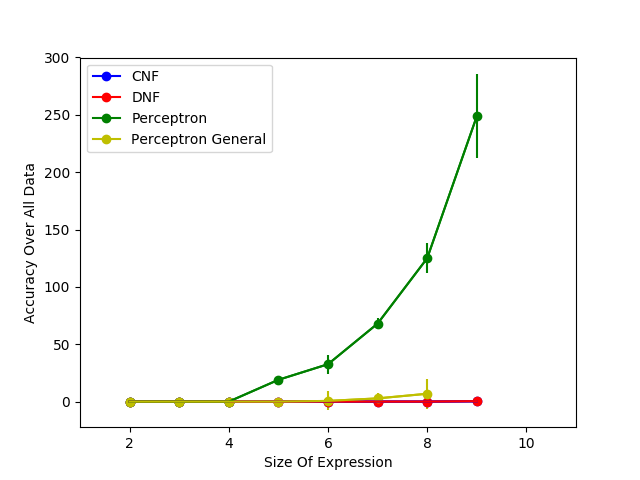
\includegraphics[width=\textwidth]{All-Peformance-Comparason.png}
    \caption{}
    \label{fig:peformance-comparason-all}
  \end{minipage}
  \hfill
\end{figure}

\begin{figure}[H]
  \centering
  \begin{minipage}[b]{0.8\textwidth}
    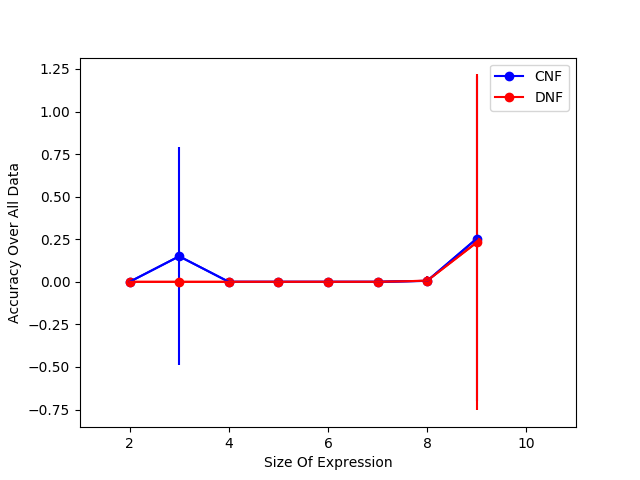
\includegraphics[width=\textwidth]{CNFvsDNF.png}
    \caption{}
    \label{fig:peformance-comparason-cnfdnf}
  \end{minipage}
  \hfill
\end{figure}

Figure  \ref{fig:peformance-comparason-all} shows that neither of the perceptron networks perform as well as the LNF Networks as $n$ increases. Figure  \ref{fig:peformance-comparason-cnfdnf} shows on average there are no statistically significant differences between the CNF or DNF networks. What is not present in  \ref{fig:peformance-comparason-cnfdnf} is that at $n = 9$ sometimes the CNF network far out performs the DNF and visa versa, theoretically both should be able to learn any boolean expression, this is something which will be investigated, as identified in the Chapter \ref{C:futureplan}. 

\section{LNF Network Generalization}
These networks are able to perform as well as standard perceptron networks but so far they have been getting the complete set of data, in practice this will almost never be the case. Standard ANN's are widely used because of their ability to generalize, for LNFN's to be useful they must also be able to generalize.

\begin{figure}[H]
	\centering
	\begin{minipage}[b]{0.8\textwidth}
		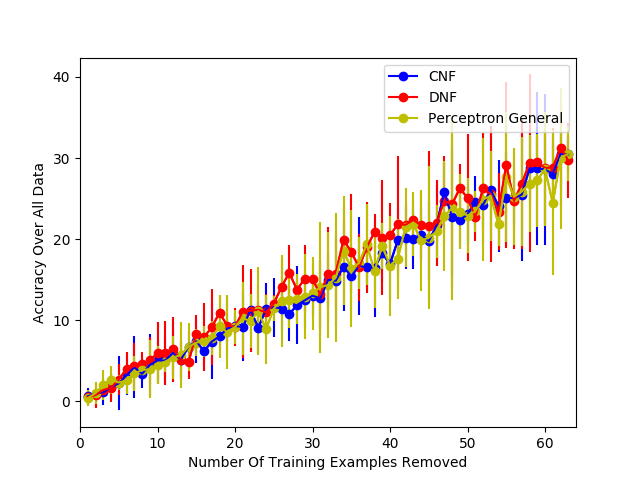
\includegraphics[width=\textwidth]{6-generalization.png}
		\caption{}
		\label{fig:generalization-peformance-6}
	\end{minipage}
	\hfill
\end{figure}

Figure \ref{fig:generalization-peformance-6} shows a comparison between the generalization ability of CNF, DNF and Perceptron networks. The graph shows the performance over all training data when successively removing elements from the training set. It demonstrates that the CNF and DNF networks generalize as well as the perceptron networks when the boolean formula has 6 inputs, this trend continues as n increases up to 9.

\section{LNF Network Rule Extraction}
The goal of this report is to learn rules which can be extracted from the network, consequently a method must be developed to extract the rules from LNF Network's. Take the weights of a trained LNFN, these weights can be converted back into $\epsilon_i$'s by apply the sigmoid function to each $w_i$.\\

As $\epsilon_i \rightarrow 0$ then $x_i$ becomes relevant and as $\epsilon_i \rightarrow 1$ then $x_i$ becomes irrelevant. If the network has learned the correct DNF or CNF representation the for every neuron if input $i$ is relevant then $w_i \rightarrow -\infty$ and therefore $\epsilon_i \rightarrow 0$, otherwise $x_i$ is irrelevant and  $w_i \rightarrow \infty$ meaning $\epsilon_i \rightarrow 1$.\\

Consequently in $\epsilon$ form the weights of the LNFN are almost binary (i.e. very close to 0 or 1) and rules can be easily extracted as a boolean formula. Many clauses in the extracted expression contain redundant terms, i.e. clauses that are a tautology or a duplicate of another, filtering these out is not an expensive operation.\\

When training an LNFN over the entire truth table for a boolean expression, when a low error is achieved it is possible to extract boolean formula from the network which gets can generate the original truth table. This is a necessary first step but a more important question is, can formula still be extracted from the network when the LNFN is not trained with the entire truth table? If it can then what does this formula represent?

\chapter{Conclusion}\label{C:con}

\comment{Talk about final applications here when they have been finished}

This report demonstrated that Logical Normal Form Networks (LNFNs) had statistically equivalent performance and generalization to Multi-Layer Perceptron Networks when trained over a number of randomly generated truth tables. LNFNs where shown to learn a representation which corresponded to a correct boolean formula, this formula was also able to generalize.\\

While LNFNs have these nice properties there are significant down sides which result in them being impractical. The critical issue is that they require $2^n$ hidden neurons.\\

A generalized version of LNFNs called Logical Neural Networks (LNNs) where introduced and improved apon to get a improvement in performance. LNNs where then shown to have more interpretable weight by training different network structures on the MNIST data set.\\

Finally ...



%%%%%%%%%%%%%%%%%%%%%%%%%%%%%%%%%%%%%%%%%%%%%%%%%%%%%%%

\backmatter

%%%%%%%%%%%%%%%%%%%%%%%%%%%%%%%%%%%%%%%%%%%%%%%%%%%%%%%


%\bibliographystyle{unsrt}
\bibliographystyle{ieeetr}
\bibliography{sample}

\begin{appendices}
\chapter{Proposal}
\section*{1. Introduction}

Neural Networks (NN's) perform exceptionally well over a wide range of different problems. However once trained these networks become a black box, near impossible for a human to interpret the learned representation and understand patterns in the features identified by the NN. 

Logical Neural Networks (LLN's) are NN's with activation functions which resemble logic gates. The idea being that if we are able to think about the output of neuron as a logical combination of inputs and weights then prehaps we can understand the learned structure of the network.

LNN's, have previously been shown to provide a simpler representation while still performing well \cite{LearningLogicalActivations} (in the context of the MINST data set). Despite the promise of LNN's they have not been deeply explored.

\section*{2. The Problem}

LNN's are an exciting concept because of their interpretability, this combined with their reasonable performance (when compared to standard NN's) makes them a promising solution to the usual "black boxeyness" of NN's. We suggest this problem still hasn't been solved as we have yet to develop a foundation for LNN's. First we ask, can it be demonstrated through experementation that like standard NN's, LNN's are also universal function approximators?  Before we can hope to answer this key question we also must ask whether we have the right parametrization of logical gates as these form the foundation of an LNN. \\

Regardless of our answer to the first question a next logical step for our investigation is to ask, what types of problems is an LNN best suited to? Which ones can it not only perform well on but also provide a interpretable learned representation. This will help build the foundation of LNN's, giving us a better understanding of how to configure them for different problems, i.e. network layout and which logical neurons to use.\\

\section*{3. Proposed Solution}

To begin this project we take a step back to ensure we have the right approach. A network built out of neurons that resemble logic gates we would expect should be able to learn any given boolean formula. This would show we have good paramaterisations for our logical gates and be a fundamental step towards showing LNN's are universal function approximators. First we must address a key issue with our existing setup, namely our choice of "gates" is not a functionally complete set. So far LNN's have been shown to perform with a reasonable accuracy on the MINST data set using layers consisting of only Noisy-OR and Noisy-AND neurons. Consider the problem of representing some known boolean expression using discrete logic circuit, but we only have access to AND and OR gates. These two gates combined does not make a functionally complete set. We propose to implement a number of different sets of functionally complete neurons, such as NAND and NOR. If an LNN consisted of multiple layers of NAND's or NOR's we would expect to find groups of gates learning to act like some of our other gates. One issue we might encounter here is that there is a set of weights which allows a given network to represent a given boolean expression but the network is unable to learn these weights. The gates we aim to paramaterise and implement are AND, OR, NOT, NAND, NOR. \\

The first 4 weeks of this project would be taken to fully understand the concept of Noisy gates, using the bibliography of the previous research and other resources, along with developing our paramaterisation of logical gates. By the end of this we will have produced a bibliography and our gate paramaterisations.\\

We would like to demonstrait that we can use our logical neurons to learn any given boolean expression (if we have an arbarary number of neurons). We will design experements by generating some boolean expressions and then simply feeding the expression into a LNN. It would be interesting to also feed these expressions into a standard NN for a comparason in peformance. We might find that inpractice that some boolean expressions cant be learnt, in this case we will investigate and provide justification for this outcome. During these experements we can also identify what training data will yeild a LNN which generalises effectively i.e. can we fix an input variable to be only 0 while training and obtain a network which generalises to the case where that variable  is 1? We expect to spend 7 weeks investigating and running experements at the conclusion of which we will have evedience allowing us to provide an answer to our question.

Next we address a fundamental question, are LNN's universal function approximators? We design experements in a similar fassion as before except this time rather than being boolean expressions we will generate integer and real valued functions, similarly comparing peformance to standard NN. We allocate 7 weeks for this section, at the conclusion of which we will have evidence to provide an answer to the question posed above. \\

Now that we will have explored the foundation of LNN's, using what we have discovered we can use our LNN to solve standard benchmark problems and compare against performance of standard NN's. We would use K-Fold Cross Validation, which is commonly used for comparisons like this. It would then be useful to examine the trained LNN's and see if we can interpret how the network has learned to solve the problem. This is a logical place to return to as this really is the motivation behind LNN's. We allocate 5 weeks for this. \\

An overview of the proposed solution follows
\begin{itemize}
	\item Produce bibliography and paramaterisation of gates (est: 5 weeks)
	\item Demonstraiting LNN's are/are not able to learn any known boolean function (est: 7 weeks)
	\item Demonstraiting LNN's are/are not universal function approximators (est: 7 weeks)
	\item Evaluate LNN's on benchmark problems (est: 5 weeks)
\end{itemize}
This only allocates 24 weeks, the left over time is to account for slippages.


\section*{4. Evaluating your Solution}

A solution to this problem should build the foundation to LNN's. Giving strong evedience through experements that LNN's can or cant learn any known boolean function and strong evidence showing that LNN's are or are not universal function approximators. This would require an in depth investigation into various paramaterisations of logic gates. Following this it should identify where LNN's are most powerful and where a standard NN should be used instead. Finally a comparason of accuracy and interpretability of LLN's against standard NN's over various benchmark problems.

\section*{5. Resource Requirements}

I do not for see any requirements I don't already have access to.
	
\end{appendices}


\end{document}
